%------------------------ Packages ------------------------
\documentclass[12pt,a4paper]{article}
\usepackage[latin1]{inputenc}
\usepackage[T1]{fontenc}
\usepackage[pdftex]{graphicx}
\usepackage{float}
\usepackage{amsmath}
\usepackage{amssymb}
\usepackage[FIGTOPCAP]{subfigure}
\usepackage{color}
\usepackage[hidelinks]{hyperref}

\newcommand{\version}{\IfFileExists{../../version.txt}
{\input{../../version.txt}}
{\input{../../../version.txt}}
}

\newcommand{\command}[1]{%
\indent \fcolorbox{black}{white}{%
   \begin{minipage}{\dimexpr\textwidth-\parindent\relax}%
      #1
   \end{minipage}%
}
}

\newsavebox{\FVerbBox}
\newenvironment{sample}
{\par \vspace{0.2cm} \begin{lrbox}{\FVerbBox}
\begin{minipage}{\dimexpr\textwidth-\parindent\relax}}
{\end{minipage}
\end{lrbox}
\fcolorbox{black}{lightgray}{\usebox{\FVerbBox}}
\vspace{0.2cm}}

\newenvironment{sampletitle}
{\vspace{0.2cm} \noindent\textbf{Example} :
\begin{sample}}
{\end{sample}}

\newcommand{\samplecomment}[1]{%

\textit{#1}
}

\newcommand{\seealso}[1]{\vspace{0.2cm} \noindent\textbf{See also} :\par #1}

% tikz
\usetikzlibrary{calc}
\usetikzlibrary{arrows}
\usetikzlibrary{shadows}

\tikzset{block/.style={draw, text centered, fill=gray!10,drop shadow}}
\tikzset{connect/.style={draw, line width=1 pt}}

\begin{document}

\begin{center}
\textbf{\huge  \underline{Dynthreshold operator}}
\end{center}
\vspace{0.5cm}

The dynthreshold operator is a morphological operation used to give a constant ratio of black and white pixels with a greyscale image as the input, and a binary image as a result. The W/B pixel ratio can be set dynamically. \\

\begin{figure}[h!]
\centering
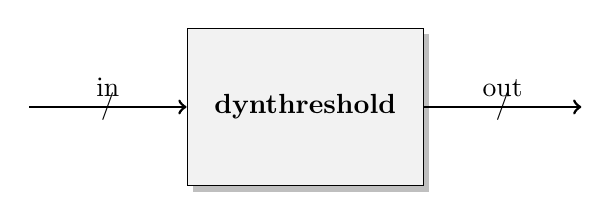
\begin{tikzpicture}
\node[block,rectangle,minimum height=2cm,minimum width=3cm] (bloc) {\textbf{dynthreshold}};

\path[connect,<-] ([yshift=0.0cm]bloc.west) -- node{/} node[above]{in} ++(-2cm,0);

\path[connect,->] ([yshift=0.0cm]bloc.east) -- node{/} node[above]{out} ++(2cm,0);
 ([xshift=0.5cm,yshift=-0.6cm]bloc.north);

\end{tikzpicture}
\end{figure}

The threshold value matching the desired W/B pixel ratio the closest is computed after several images: A first approximation is done via a dichotomic research, until the difference bewteen the targeted ratio and the current ratio is under a value defined in percent by BorderResearchType. The optimal threshold value is then reached with several increments of its value. 
The behaviour of the dynthreshold operator can be changed with the BorderResearchType slider:
\begin{itemize}
\item Increasing BorderResearchType value will slow down the threshold computing, but will also increase stability and reduce sensibility to ambient light changes.
\item Decreasing BorderResearchType value will allow to quickly approach the optimal threshold value, but also reduce stability and increase sensibility to luminosity variations. 
\end{itemize}

The first image received is binarized with a default threshold value of 0. For each image, the number of white pixels is kept, and compared to the total number of pixels. If the reached ratio is too low, the threshold is decreased to blacken fewer incoming pixels. In the same way, the threshold is increased if the obtained ratio is higher than desired.
\vspace{0.5cm}





\section*{Properties}
\properties{
enable             & bool & Enable the processing \\
DesiredRatio		   & int  & Ratio White / black pixels in percent\\
BorderResearchType  & int & Difference in percent between current ratio and desired ratio triggering the switch between dichotomic and iterative search\\
}

\vspace{0.5cm}

\section*{Constants}

\constants{
IN\_SIZE & Size of the input flow : 1 byte (greyscale image) or 1 bit (binary image)\\
OUT\_SIZE & Size of the output flow : 1 byte (greyscale image) or 1 bit (binary image)\\
}

\begin{figure}[!h]
\centering
\subfigure[Initial greyscale image]{
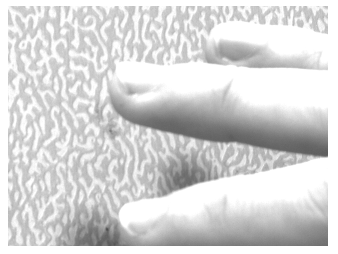
\includegraphics[width=7cm]{original.png}}
\vspace{1cm}
\hspace{3cm}
\subfigure[Binarized image]{
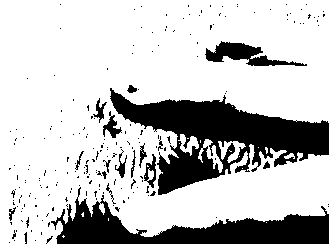
\includegraphics[width=6.5cm]{binary.png}}
\hspace{0.5cm}
\subfigure[Output with a 33\% W/B px ratio]{
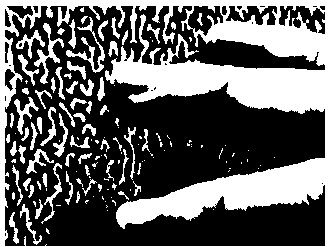
\includegraphics[width=6.5cm]{dynthreshold.png}}
\end{figure}


%
%\section*{Equivalence}
%\subsection*{Matlab}
%
%\lstset{language=Matlab}
%\begin{lstlisting}
%I; % image matrix
%SE = [0 1 0 ; 1 1 1 ; 0 1 0]; % Structural element 3x3
%I_dilated = imdilate(I,SE); % dilation operation on I with SE as a structuring element object.
%% This functions takes a grayscale or a binary image
%
%\end{lstlisting}
%
%\url{https://fr.mathworks.com/help/images/ref/imdilate.html}
%
%
%\subsection*{OpenCV}
%
%\lstset{language=C++}
%\begin{lstlisting}
%void dilate(InputArray src, OutputArray dst, 
%	InputArray kernel, Point anchor=Point(-1,-1), 
%	int iterations=1, int borderType=BORDER_CONSTANT, 
%	const Scalar& borderValue=morphologyDefaultBorderValue()
% )
%
%/*Parameters:	
%    src - input image; the number of channels can be arbitrary, but the depth should be one of CV_8U, CV_16U, CV_16S, CV_32F` or ``CV_64F.
%    dst - output image of the same size and type as src.
%    element - structuring element used for dilation; if element=Mat() , a 3 x 3 rectangular structuring element is used.
%    anchor - position of the anchor within the element; default value (-1, -1) means that the anchor is at the element center.
%    iterations - number of times dilation is applied.
%    borderType - pixel extrapolation method (see borderInterpolate() for details).
%    borderValue - border value in case of a constant border (see createMorphologyFilter() for details).
%*/
%\end{lstlisting}
%
%\url{http://docs.opencv.org/2.4/modules/imgproc/doc/filtering.html#dilate}
%
%\section*{Mathematical formalism}
%
%The operator uses a $3x3$ binary kernel called "Structuring element" which is giving the neighbours to evaluate around each point of the image. \\
%
%The generalization of dilation to gray-level images is that the gray-level value at any point is replaced by the $maximum$ intensity value covered by the flat structuring element. That is, pointwise dilation of the image $I$ by a flat structuring element $SE$ is defined as:\\
%
%
%\centering
%$\displaystyle I \oplus SE (\bf x )$ 	$\textstyle =$ 	$\displaystyle max \{I({\bf z}): {\bf z} \epsilon S_x \},$
%
%\vspace{0.5cm}



\end{document}